\section{Облік доказів та обмежена перевірка}
\label{sec:evidence}

Доказовий шар розділяє твердження джерела, його архівоване подання та подальшу оцінку. Конкретною реалізацією є клас Python \code{EvidenceLedger}, який зберігає версіоновані записи JSON у SQLite. Назви записів у таблиці~\ref{tab:evidence} позначають дискримінатори словників, а не сім відповідних класів Python. Функції аналізу окремо обмінюються JSON-сумісними документами, валідованими за схемами. Їхні зв'язки походження концептуально споріднені з PROV, але експорт RDF чи відповідність PROV-O не продемонстровано \citep{moreau2013provdm,lebo2013provo}.

\begin{table}[!htbp]
\centering
\small
\caption{Конкретні види записів реєстру та забезпечувані межі. Посилальна цілісність встановлює простежуваність, але не встановлює доказового логічного випливання.}
\label{tab:evidence}
\begin{tabularx}{\linewidth}{@{}lXX@{}}
\toprule
Вид запису & Збережений вміст і зв'язки & Основне структурне обмеження \\
\midrule
Source & URI, назва, видавець, час публікації & Ідентифікатор і обов'язкові метадані \\
Artifact & Зв'язок із джерелом, шлях, дайджест, час збору & Наявне джерело; синтаксис SHA-256 \\
Passage & Зв'язок з артефактом, текст, локатор & Наявний артефакт; непорожній текст \\
Claim & Твердження, тип, зв'язки з джерелами й доказами & Атрибутоване джерело або докази висновку \\
ClaimMention & Зв'язки із твердженням та уривком & Оприлюднене твердження й уривок із того самого джерела \\
EvidenceAssessment & Твердження, статус, докази, обґрунтування & Дійсні посилання й ланцюг заміщення \\
VerificationResult & Обсяг, гранична дата, статус, сторони доказів & Узгоджені зі статусом посилання на докази \\
\bottomrule
\end{tabularx}
\end{table}

Реєстр відхиляє оновлення й видалення через тригери SQLite. Повторне вставлення ідентичного запису ідемпотентне; повторне використання ідентифікатора з іншим вмістом завершується помилкою. Оцінки й результати перевірки можуть заміщувати попередні записи, не замінюючи їх, причому заміщення має стосуватися того самого твердження й не може розгалужуватися. Дайджест артефакта перевіряється за форматом, а не обчислюється реєстром заново з архівованого файлу. Локатор уривка може містити довільний JSON; перевірка точного текстового фрагмента належить окремому конструктору оцінки. Ці розрізнення показано на рисунку~\ref{fig:provenance}.

\begin{figure}[!htbp]
\centering
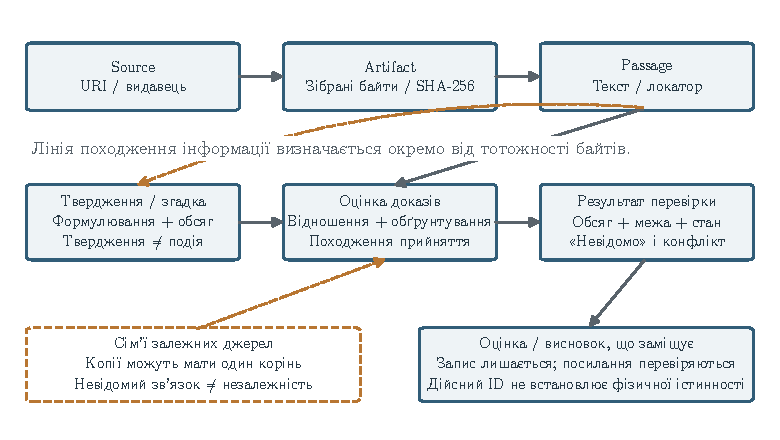
\includegraphics[width=\linewidth]{evidence_provenance.pdf}
\caption{Зв'язки доказів і походження. Твердження джерел, байти артефактів, виділені уривки й аналітичні судження лишаються окремими. Зафіксована лінія походження й дійсні локатори підтримують перевірку, але не гарантують істинності чи незалежності джерел.}
\label{fig:provenance}
\end{figure}

Локальний пошук використовує BM25 на наданих уривках, шукає в напрямах твердження та контрдоказів і дотримується граничного часу збору й бюджету запитів. Результати лишаються неоціненими кандидатами. Конструктор оцінки перевіряє, що цитований фрагмент у кодових точках Unicode дорівнює підрядку уривка, валідує обсяг і числові обмеження та фіксує походження прийняття. Прийняті оцінки потребують мітки людського рішення або мітки валідованого правила з ідентифікатором правила. Це структурна вимога: конструктор не звертається до незалежно валідованого реєстру правил. Спеціалізований збирач тверджень надає другу мітку програмно.

Спільний словник перевірки містить сім станів: \code{unverified}, \code{supported_within_scope}, \code{refuted_within_scope}, \code{conflicting_evidence}, \code{insufficient_evidence}, \code{not_verifiable} і \code{superseded}. Він виключає оцінки, що є лише кандидатами, не відповідають часу чи обсягу або неналежно процитовані. Пороги вердикту рахують оголошені ідентифікатори ліній походження; окремі поля рахують корені, явно позначені як незалежно підтверджені. Ці величини не можна змішувати. Обсяг фізичного факту додатково вимагає прийнятої прямої фізичної доказової основи, перш ніж підтримка чи спростування можуть бути чинними. Тому заперечення установ може лишатися зафіксованим як офіційна позиція, тоді як доказів фізичного твердження бракує. Цей запобіжник залежить від наданого типу обсягу; він незалежно не класифікує епістемічний обсяг твердження.

Кураторський пакет кейсу містить 25 тверджень, 25 обраних уривків і 36 прийнятих оцінок за правилом. Його поточні результати за схемою~2.3 --- 19 підтриманих, нуль спростованих і шість із недостатніми доказами. Це вихідні дані програми, а не вимірювання точності. Раніший пакет за схемою~2.0 давав 21 підтриманий і чотири спростовані результати з 31 оцінки, вставляючи визначені уривки й очікувані відношення в побудову оцінок. Поточний код оцінює лише знайдених кандидатів і усуває це пряме вставлення, але твердження, запити, уривки, обсяги й мітки ліній походження лишаються кураторськими. Загальний офлайн-запускач обмеженіший: він шукає кандидатів і не створює прийнятих оцінок.

Два спеціально сконструйовані випробування показують семантичні збої базового зіставлювача; пізнішу ревізію оцінено в розділі~\ref{sec:rule-v2}. Уривок про 26 дерев приймається як підтримка твердження про 26 військових у будівлі, а речення із запереченням прибуття поліції --- як підтримка прибуття. Обидва отримують фіксовану впевненість гілки 0,92. Збережений артефакт кейсу також приймає уривки про травми й самостійне пересування як підтримку твердження про чотирьох осіб, які самовільно залишили частину. Збіг чисел може задовольнити правило підтримки без збігу присудка, а лексичне перекриття може пропустити звичайне заперечення. Крім того, висновок використовує весь уривок, тоді як збережена цитата може бути коротшим знайденим фрагментом. Тому точне цитування не гарантує, що цитата логічно обґрунтовує призначене відношення.

Жоден незалежний локальний еталонний набір не встановлює точності логічного випливання й не калібрує ці значення впевненості. Випробування демонструють збої, а не оцінюють їх поширеність. FEVER і AVeriTeC обґрунтовують спільне оцінювання достатності доказів і правильності вердикту \citep{thorne2018fever,schlichtkrull2023averitec,schlichtkrull2024averitec}, але не замінюють оцінювання цієї системи на незалежно встановлених твердженнях. InFact є зовнішнім поетапним орієнтиром \citep{rothermel2024infact}, а не виміряною тут базовою лінією.
